\documentclass[10pt, hyperref={pdfpagelabels=false}]{beamer}

\usepackage{lmodern}
\usetheme{Boadilla}
\setbeamertemplate{navigation symbols}{}

\usepackage{booktabs}
\usepackage{graphicx}
\usepackage{appendixnumberbeamer}
\usepackage{amsmath}

% Colors
\definecolor{mygreen}{RGB}{48, 132, 42}
\definecolor{myblue}{RGB}{94, 103, 209}
\definecolor{mygray}{gray}{0.5}

% Section transition slide command
\newcommand{\sectionslide}[1]{%
  \begin{frame}
  \vfill
  \begin{center}
  {\Large \textcolor{myblue}{\textbf{#1}}}
  \end{center}
  \vfill
  \end{frame}
}

% Title info
\title[Decentralization \& Gangs]{Decentralization and Criminal Gangs in El Salvador: \\ Impacts on Municipal Finances and Local Economic Development}

\author[Jose Larios]{Kent Eaton\inst{1} \and Silvana Huanqui\inst{2} \and \textbf{Jose Larios}\inst{3}}

\institute[]{\inst{1}University of California, Santa Cruz \and \inst{2}Universidad del Pac\'ifico, Lima \and \inst{3}Georgia State University, Andrew Young School of Policy Studies}

\date[Georgia State University, 03/26/2026]{Georgia State University \\ 03/26/2026} %% <-- PLACEHOLDER: Replace with venue and date

\begin{document}

%%%%%%%%%%%%%%%%%%%%%%%%%%%%%%%%%%%%%%%%
%            TITLE PAGE                %
%%%%%%%%%%%%%%%%%%%%%%%%%%%%%%%%%%%%%%%%

\begin{frame}
\titlepage
\end{frame}


%%%%%%%%%%%%%%%%%%%%%%%%%%%%%%%%%%%%%%%%
%  SECTION 1: INTRODUCTION            %
%%%%%%%%%%%%%%%%%%%%%%%%%%%%%%%%%%%%%%%%

\sectionslide{Introduction}


%***************************************%
\begin{frame}{Motivation}

\begin{itemize}

\item Decentralization played a key role in El Salvador's post-civil war transition (1992 onward).\\
\vspace{0.25cm}
\begin{itemize}
\item Municipalities became spaces of political contestation.\\
\item FMLN won local elections $\Rightarrow$ foundation for national victories.\\
\item Participatory mechanisms broadened decision making.
\end{itemize}

\pause
\vspace{0.25cm}
\item More recently, a different non-state armed actor has undermined this progress: \textcolor{myblue}{\textbf{criminal gangs (maras)}}.\vspace{0.25cm}
\begin{itemize}
\item MS-13 and Barrio 18: up to 60,000 members.
\item Operated in nearly all 262 municipalities.
\item Widespread extortion of households and businesses.
\end{itemize}

\end{itemize}
\end{frame}


%***************************************%
\begin{frame}{This Paper}

\begin{block}{Key Question}
How does the presence of criminal gangs affect the performance of decentralized institutions?
\end{block}

\pause

\begin{itemize}

\item Existing literature: decentralization $\Rightarrow$ leverage for gangs (Rios, 2013; Dur\'an-Mart\'inez, 2018).

\item We \textcolor{myblue}{\textbf{reverse the causal arrow}}: gangs $\Rightarrow$ undermine decentralization.

\pause

\item \textbf{Findings:}
\begin{itemize}
\item Gang presence \textcolor{red}{reduces} own-source revenues (especially mid-size municipalities).
\item Gang presence \textcolor{red}{reduces} municipal spending and service provision.
\item Gang presence \textcolor{red}{reduces} local economic activity, with \textcolor{red}{spillovers} to neighboring municipalities.
\end{itemize}

\end{itemize}
\end{frame}


%***************************************%
\begin{frame}{Fit in the Literature}

\textbf{Gangs and the state: symbiosis or parasitism?}

\begin{itemize}

\item[\textcolor{mygray}{\textbullet}] \textcolor{mygray}{Blattman et al.\ (2021): Gangs provide governance to protect drug rents $\Rightarrow$ complementarity with the state.}

\item[\textcolor{mygray}{\textbullet}] \textcolor{mygray}{Lessing (2021): Criminal governance as complement to state governance.}

\item[\textcolor{mygray}{\textbullet}] \textcolor{mygray}{Di Cataldo \& Mastrorocco (2021): Organized crime distorts public service provision.}

\end{itemize}

\pause

\begin{block}{Our contribution}
In El Salvador, gangs do \textbf{not} rely on drug trafficking $\Rightarrow$ no incentive to provide order. Instead, heavy reliance on \textcolor{myblue}{\textbf{extortion}} creates a \textcolor{red}{\textbf{parasitic}} relationship that hollows out municipal governance.
\end{block}

\end{frame}


%***************************************%
\begin{frame}{Mechanisms}

Gangs disrupt the causal mechanisms behind decentralization's benefits:

\bigskip

\begin{tabular}{lcp{6cm}}
\textcolor{myblue}{Factor mobility} & $\Rightarrow$ & Checkpoints, extortion on transport of goods \\
\\
\textcolor{myblue}{Own-source revenue collection} & $\Rightarrow$ & Competing ``taxation'' by gangs \\
\\
\textcolor{myblue}{Service provision} & $\Rightarrow$ & Territorial control limits municipal operations \\
\\
\textcolor{myblue}{Local economic activity} & $\Rightarrow$ & Extortion raises costs, depresses production \\
\end{tabular}

\end{frame}


%%%%%%%%%%%%%%%%%%%%%%%%%%%%%%%%%%%%%%%%
%  SECTION 2: DECENTRALIZATION IN SV  %
%%%%%%%%%%%%%%%%%%%%%%%%%%%%%%%%%%%%%%%%

\sectionslide{Decentralization in El Salvador}


%***************************************%
\begin{frame}{Institutional Design}

\begin{itemize}

\item Unitary state with \textbf{262 municipalities} (only subnational level).

\item \textbf{Political}: Majoritarian electoral rules; since 2015, some opposition seats on council.

\item \textbf{Fiscal}:
\begin{itemize}
\item No municipal property tax.
\item Own-source revenues: fee-based taxes on economic activities, user fees, sale of goods/services.
\item Transfers: FODES (Fund for Municipal Economic and Social Development), since 1988.
\item FODES rule: 80\% capital investment, 20\% operating expenses.
\end{itemize}

\item \textbf{Administrative}: Trash collection, local policing, housing, transport regulation, local economic development.

\end{itemize}
\end{frame}


%***************************************%
\begin{frame}{Municipal Finances: Key Facts (2010--2018)}

\begin{itemize}
\item High reliance on transfers: FODES $\approx$ 48\% of total municipal revenues.
\item Low own-source revenues $\approx$ 37\% of total revenues.
\item Enormous heterogeneity by municipality size:
\begin{itemize}
\item Small municipalities: FODES = 10$\times$ own-source revenues.
\item Medium: FODES = 3.5$\times$ own-source revenues.
\item Large: FODES = 1.2$\times$ own-source revenues.
\end{itemize}
\end{itemize}

\bigskip

\begin{center}
  Per capita tax collection and size of FODES transfers, 2011--2018 \\
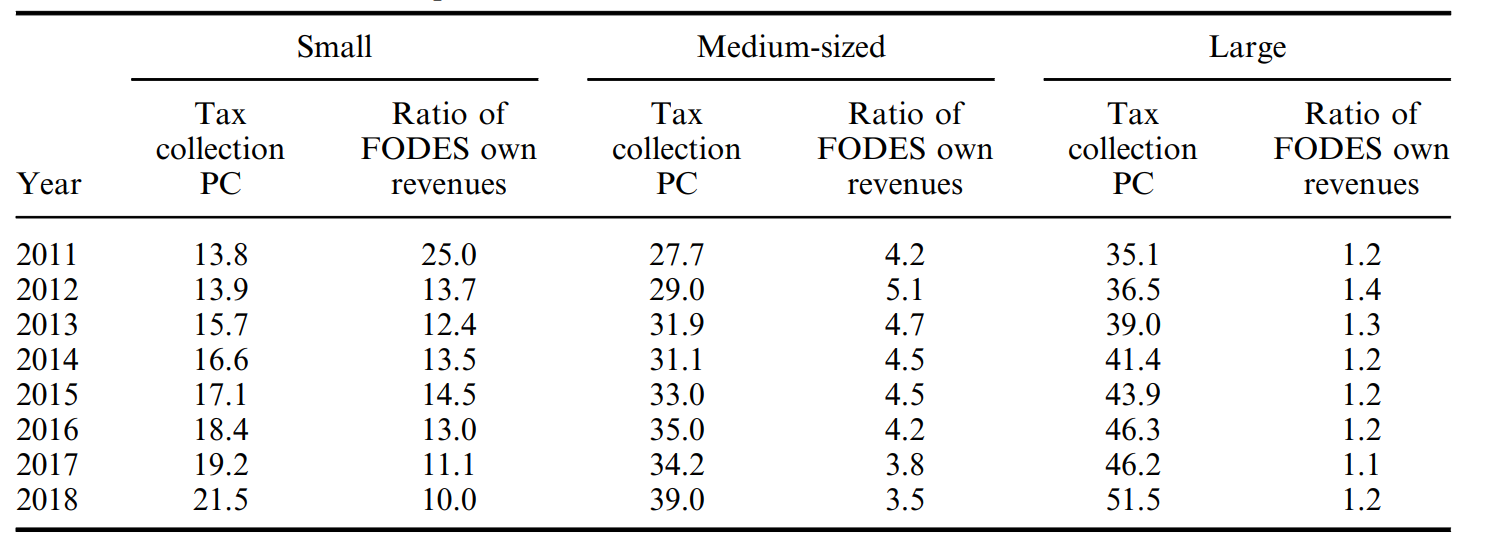
\includegraphics[width=0.85\textwidth]{Table1.png}
\end{center}

\end{frame}


%***************************************%
\begin{frame}{Own-Source Revenues Per Capita (2018)}


\begin{center}

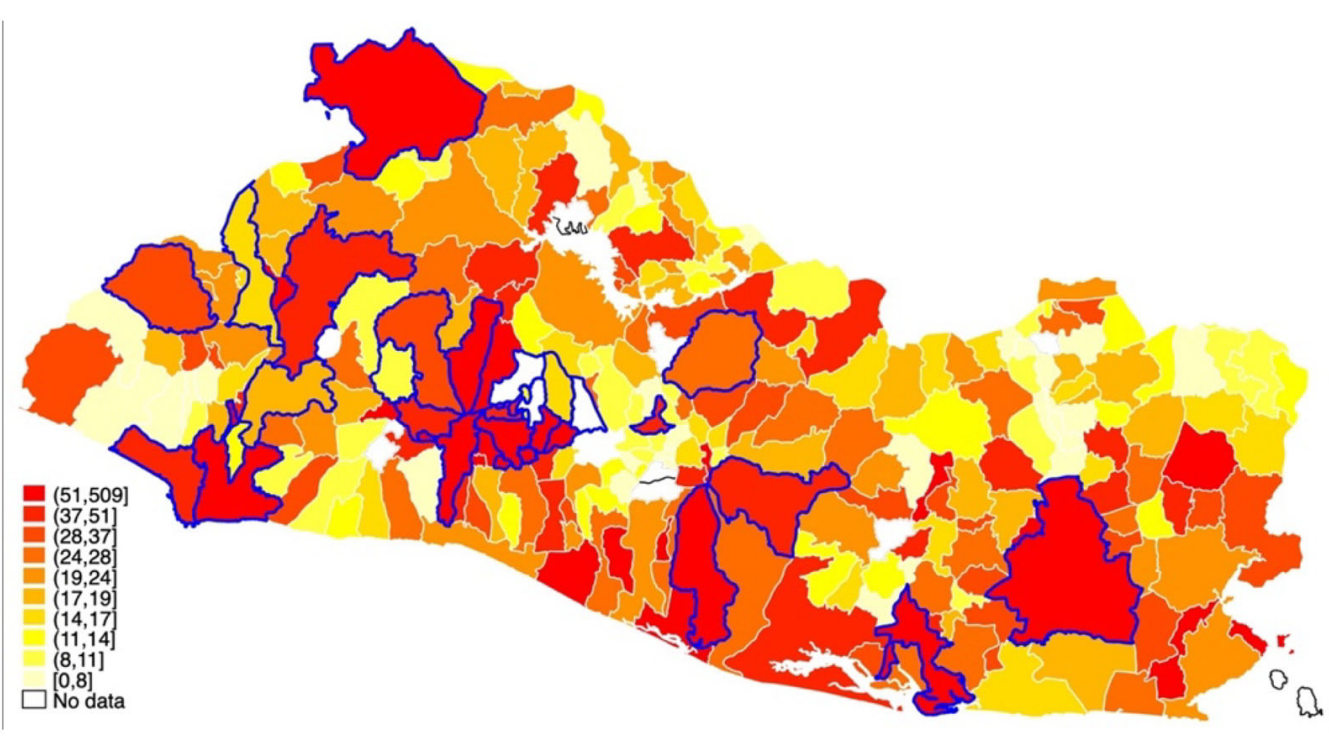
\includegraphics[width=0.85\textwidth]{Figure1.png}
\end{center}

\end{frame}


%***************************************%
\begin{frame}{Budgetary Autonomy by Department (2018)}

\begin{center}

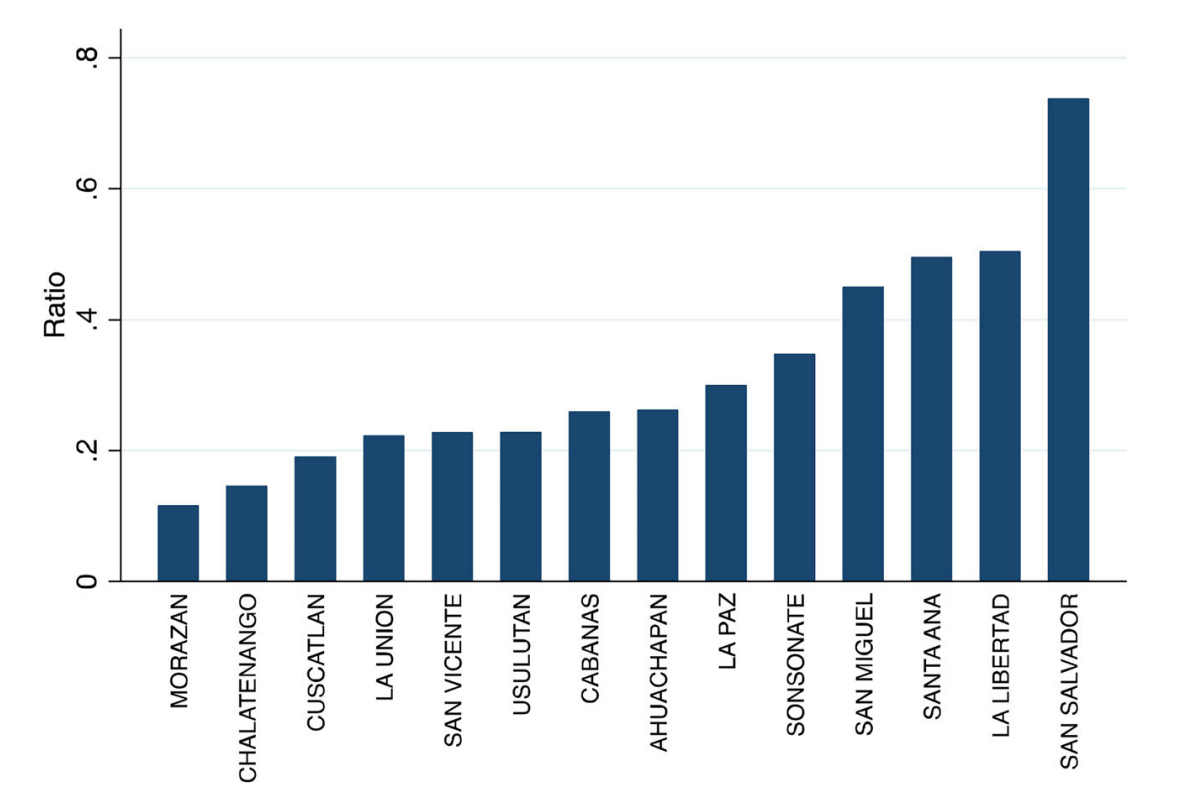
\includegraphics[width=0.85\textwidth]{Figure2.png}
\end{center}

\end{frame}



%%%%%%%%%%%%%%%%%%%%%%%%%%%%%%%%%%%%%%%%
%  SECTION 3: EMPIRICAL STRATEGY      %
%%%%%%%%%%%%%%%%%%%%%%%%%%%%%%%%%%%%%%%%

\sectionslide{Empirical Strategy}


%***************************************%
\begin{frame}{Empirical Approach}

\textbf{Panel data model with fixed effects:}
\begin{itemize}
\item 258 municipalities, 2010--2019.
\end{itemize}

\bigskip

$$Y_{i,t} = \beta_0 + \beta_1 \textit{MaraSalva}_{i,t-1} + \beta_k X_{i,t} + \sum_{t=1}^{T-1} c_t D_t + \alpha_i + \lambda_{i,t}$$

\bigskip

\begin{itemize}
\item $Y_{i,t}$: Own-source revenue p.c., expenditure p.c., public service provision.

\item $\textit{MaraSalva}_{i,t-1}$: Homicides per 1,000 inhabitants attributed to MS-13 (\textcolor{myblue}{\textbf{lagged one period}}).

\item $X_{i,t}$: Urban population, density, household income, energy consumption, capacity building.

\item Specifications by municipality size: small ($<$10k), medium (10k--50k), large ($>$50k).
\end{itemize}

\end{frame}


%***************************************%
\begin{frame}{Spatial Model for Economic Activity}

\textbf{Cross-sectional spatial autoregressive model (GS2LS):}

\bigskip

\begin{align*}
Y_i &= \beta \, \textit{Gangs}_i + \gamma \, Z_i + \theta \, W_{y,i} + \sigma \, W_{X,i} + \varepsilon_i \\
\varepsilon_i &= \lambda \, W_{\varepsilon,i} + \mu_i
\end{align*}

\bigskip

\begin{itemize}
\item $Y_i$: Electricity consumption (proxy for economic activity).
\item $W$: Spatial weights matrix (shared border = 1).
\item $\theta$: Spillover of economic activity to neighbors.
\item $\sigma$: Spillover of gang presence to neighbors' economic activity.
\item $\lambda$: Spatial autocorrelation in unobservables.
\end{itemize}

\end{frame}


%%%%%%%%%%%%%%%%%%%%%%%%%%%%%%%%%%%%%%%%
%  SECTION 4: RESULTS                 %
%%%%%%%%%%%%%%%%%%%%%%%%%%%%%%%%%%%%%%%%

\sectionslide{Results}


%***************************************%
\begin{frame}{Effect of MS-13 on Own-Source Revenues}

\begin{itemize}
\item Gang presence \textcolor{red}{reduces} own-source revenues per capita.
\item Effect driven by \textcolor{myblue}{\textbf{mid-size municipalities}} (10k--50k pop.): $-$\$5.6 per homicide/1,000 inh.
\item Not significant for small or large municipalities.
\end{itemize}
\end{frame}

%***************************************%
\begin{frame}{Effect of MS-13 violence on per capita own-source revenue}


\begin{center}

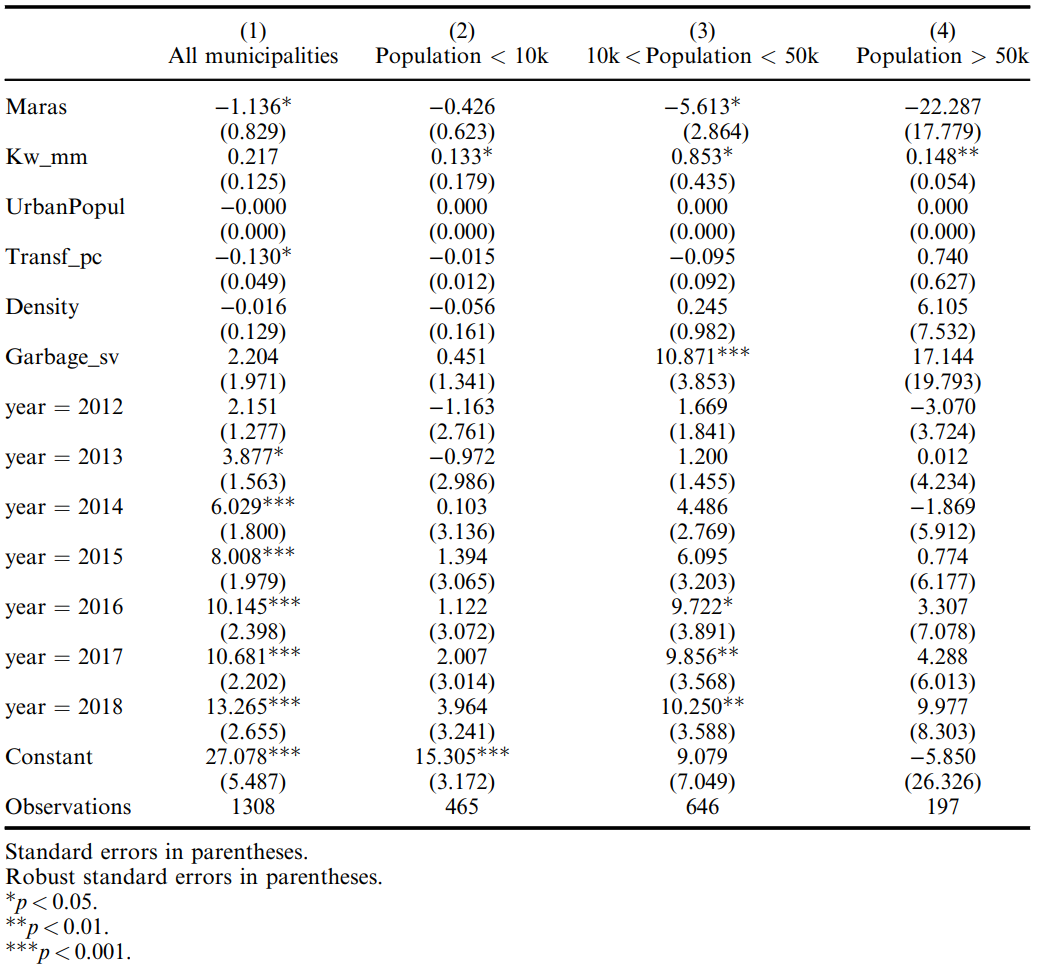
\includegraphics[width=0.7\textwidth]{Table3.png}
\end{center}

\end{frame}


%***************************************%
\begin{frame}{Effect of MS-13 on Expenditures}

\begin{itemize}
\item Significant \textcolor{red}{negative} impact on municipal spending per capita.
\item For each additional homicide/1,000 inh., expenditure drops by \$17.9.
\item Largest impact in \textcolor{myblue}{\textbf{small municipalities}}: $-$\$20 per homicide/1,000 inh.
\end{itemize}
\end{frame}
\begin{frame}{Effect of MS-13 on expenditures}
\begin{center}
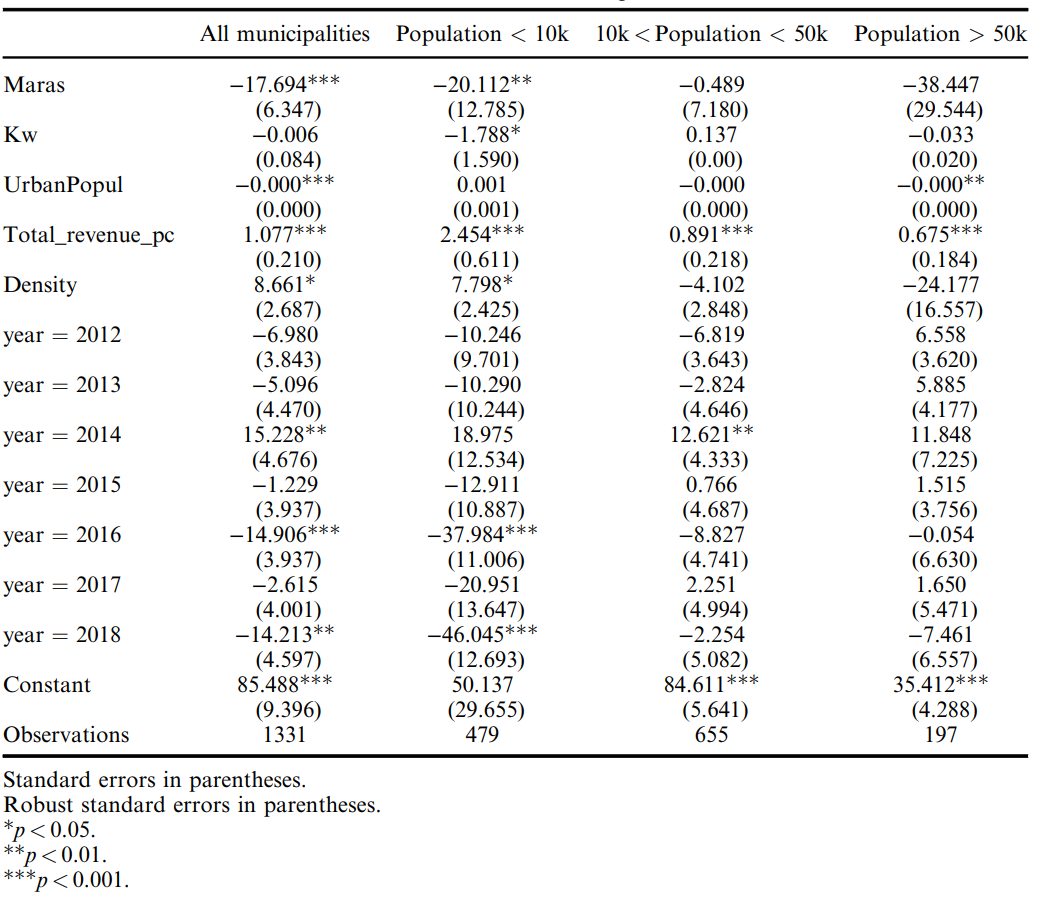
\includegraphics[width=0.75\textwidth]{Table4.png}
\end{center}

\end{frame}


%***************************************%
\begin{frame}{Current vs.\ Capital Expenditure}

\begin{itemize}
\item Capital expenditure hit hardest: $-$\$19.7 per homicide/1,000 inh.
\item Current expenditure: $-$\$2.9 per homicide/1,000 inh.
\item Effects concentrated in \textcolor{myblue}{\textbf{small municipalities}} ($<$10k pop.).
\end{itemize}
\end{frame}

\begin{frame}{Effect of MS-13 on current \& capital expenditure by size}

\begin{center}

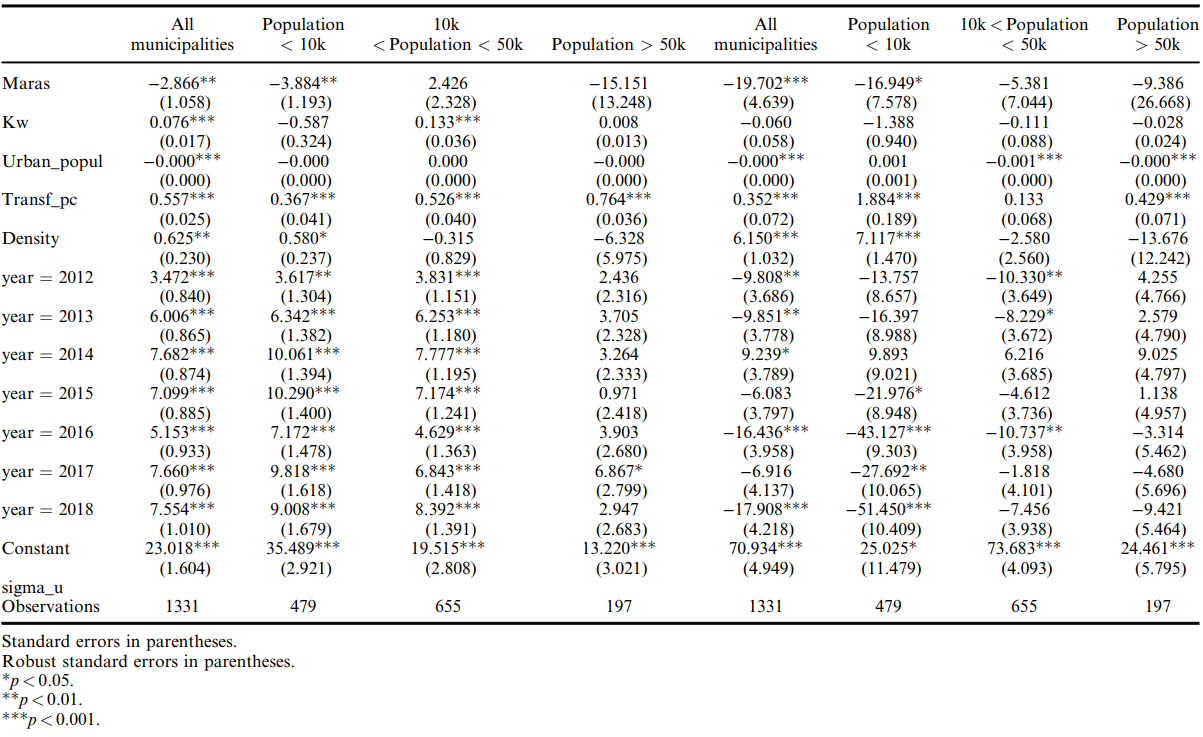
\includegraphics[width=0.95\textwidth]{Table5.png}
\end{center}


\end{frame}


%***************************************%
\begin{frame}{Effect of MS-13 on Public Service Provision}

\begin{itemize}
\item Garbage collection coverage drops by 0.2\% per homicide/1,000 inh.
\item Effect significant in \textcolor{myblue}{\textbf{mid-size municipalities}}.
\item No significant impact for small or large municipalities.
\end{itemize}

\end{frame}
\begin{frame}{Effect of MS-13 on public service provision }
\begin{center}

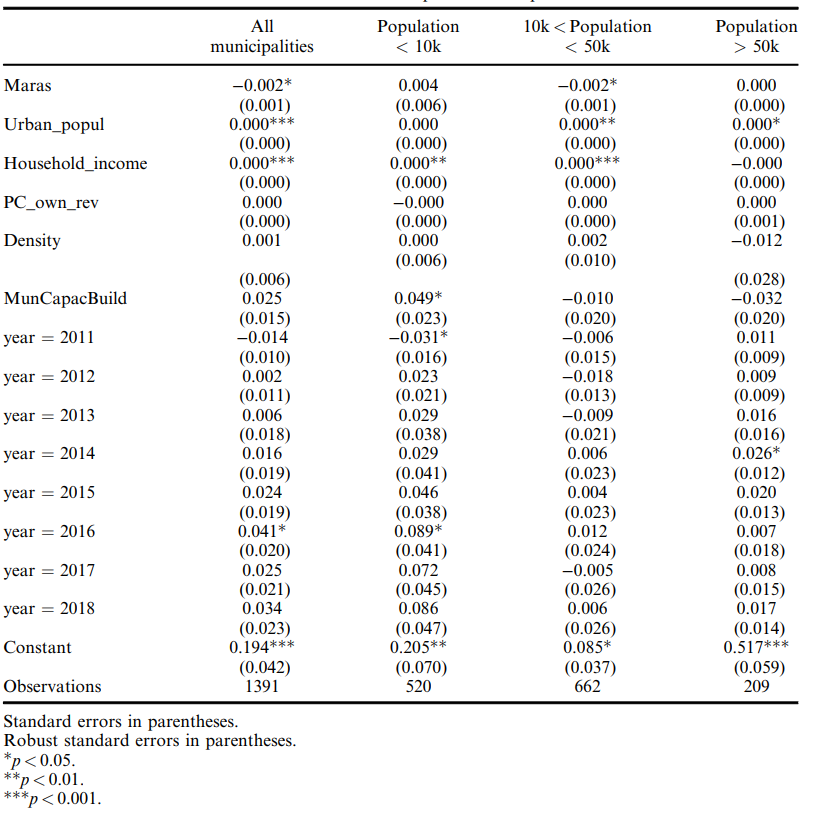
\includegraphics[width=0.65\textwidth]{Table6.png}
\end{center}

\end{frame}


%***************************************%
\begin{frame}{Effect on Local Economic Activity \& Spillovers}

\begin{itemize}
\item Each MS-13 homicide reduces local electricity consumption by \textcolor{red}{3.1 million kWh}.
\item Spillover: consumption in \textbf{neighboring} municipalities drops by \textcolor{red}{5.2 million kWh}.
\item Average municipal consumption $\approx$ 29 million kWh $\Rightarrow$ $\approx$10\% reduction.
\end{itemize}
\end{frame}
\begin{frame}{Impact of MS-13 on economic activity}
\begin{center}

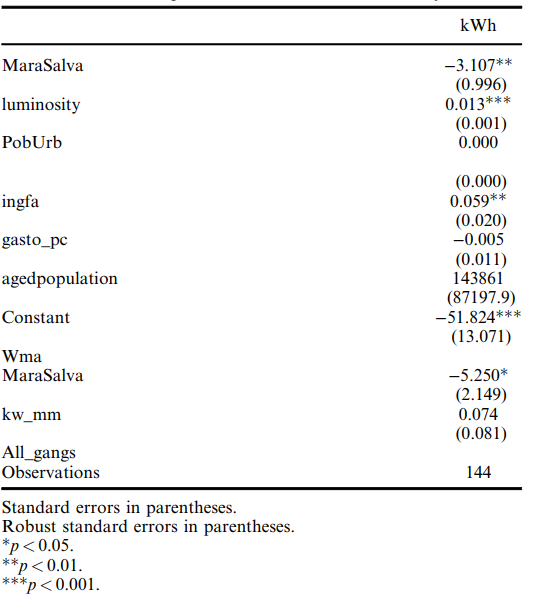
\includegraphics[width=0.5\textwidth]{Table7.png}
\end{center}



\end{frame}


%***************************************%
\begin{frame}{Robustness}

\begin{itemize}
\item \textbf{Other gangs}: Results similar when including homicides from gangs other than MS-13.

\item \textbf{2SLS / IV estimation}:
\begin{itemize}
\item Own-source revenues: MS-13 has significant negative effect (log specification).
\item Expenditures: All gangs combined show significant negative effect.
\end{itemize}

\item Results consistent across multiple specifications.
\end{itemize}

\end{frame}


%%%%%%%%%%%%%%%%%%%%%%%%%%%%%%%%%%%%%%%%
%  SECTION 5: DISCUSSION & POLICY     %
%%%%%%%%%%%%%%%%%%%%%%%%%%%%%%%%%%%%%%%%

\sectionslide{Discussion \& Policy Implications}


%***************************************%
\begin{frame}{Discussion}

\begin{itemize}

\item Gangs \textcolor{red}{hollow out} municipal governance:
\begin{itemize}
\item Lower revenues $\Rightarrow$ greater dependence on central transfers.
\item Lower spending $\Rightarrow$ reduced service provision.
\item Spillovers $\Rightarrow$ damage extends beyond gang-controlled areas.
\end{itemize}

\pause

\item Relationship is \textcolor{red}{\textbf{parasitic}}, not symbiotic:
\begin{itemize}
\item No drug trafficking $\Rightarrow$ no incentive to provide order.
\item Extortion competes directly with municipal tax collection.
\end{itemize}

\pause

\item Effects \textbf{vary by municipality size}:
\begin{itemize}
\item Mid-size: most vulnerable on revenues and services.
\item Small: most vulnerable on expenditures.
\item Large: more resilient (diversified economy, greater administrative capacity).
\end{itemize}

\end{itemize}
\end{frame}


%***************************************%
\begin{frame}{Policy Implications}

\textbf{Bukele's response}: Recentralization + militarized security.
\begin{itemize}
\item Sharp cuts in FODES transfers.
\item Central approval required for local investment.
\item Municipalities reduced from 262 to 44 (2023).
\end{itemize}

\pause
\bigskip

\textbf{Alternative: Reconstruct decentralization.}
\begin{itemize}
\item Modernize the municipal tax code $\Rightarrow$ introduce \textcolor{myblue}{\textbf{urban property tax}} (less subject to extortion).
\item Revise FODES formula $\Rightarrow$ aid mid-size municipalities most vulnerable to extortion.
\item Insulate Municipal Works Directorate from political pressure $\Rightarrow$ technocratic criteria for investment.
\end{itemize}

\pause
\bigskip

\begin{block}{}
Don't abandon decentralization --- \textbf{refine it} and exploit complementarities with the national government.
\end{block}

\end{frame}


%***************************************%
\begin{frame}
\vfill
\begin{center}
{\Large \textcolor{myblue}{\textbf{Thank You}}}

\end{center}
\vfill
\end{frame}


\end{document}
